\documentclass[a4paper, 12pt]{report}


\usepackage[czech]{babel} % czech language
\usepackage{amssymb} % for math symbols
\usepackage{amsmath} % for math symbols
\usepackage{pdfpages} % for including pdf files
\usepackage{microtype} % better text rendering
\usepackage[T1]{fontenc} % better text rendering
\usepackage{graphicx} % for images
\usepackage[hidelinks]{hyperref} % for clickable links, hidelinks hides the ugly boxes
\usepackage[a4paper,width=160mm,top=25mm,bottom=25mm,bindingoffset=6mm]{geometry} % page layout
\usepackage[pagestyles]{titlesec} % for customizing chapter titles
\usepackage{parskip} % for no indent and space between paragraphs
\usepackage{enumitem} % for customizing lists
\usepackage{fancyhdr} % for customizing headers and footers
\usepackage{bm} % for bold math symbols
\usepackage{tocloft} % for customizing table of contents
\usepackage{multicol} % for multiple columns
\usepackage{hyperref} % for clickable links
\usepackage{textcase} % for uppercasing text
\usepackage{tikz} % for drawing
\usepackage{float} % for floating images
\usepackage{siunitx} % for SI units
\usepackage{caption} % for customizing captions
\usepackage{hhline} % for double lines in tables
\usetikzlibrary{shapes.geometric} % for drawing

% toc font
\renewcommand{\cfttoctitlefont}{\normalfont\Huge\sffamily\bfseries}
\renewcommand{\cftchapfont}{\sffamily\normalsize}
\renewcommand{\cftsecfont}{\sffamily\normalsize}



% for customizing bibliography title
\addto{\captionsczech}{\renewcommand{\bibname}{Seznam zdrojů}}

\fancypagestyle{plain}{
    \renewcommand{\headrulewidth}{0pt}
    \fancyhf{}
    \fancyfoot[C]{\sffamily\selectfont--~\thepage~--}
}

\pagestyle{plain}
\fancyhead{}
\fancyhead[R]{\sffamily\rightmark}
\fancyhead[L]{\sffamily\thechapter\ \chaptername}
\setlength{\headheight}{15pt}
\renewcommand{\headrulewidth}{0.4pt}

\renewcommand{\sectionmark}[1]{\markright{#1}}

% for customizing chapter titles
\titleformat{\chapter}[display]{\normalfont\sffamily\bfseries}{}{0pt}{\Huge}

% for customizing section titles
\titleformat{\section}{\normalfont\Large\sffamily\bfseries}{\thesection}{1em}{}

% for customizing subsection titles
\titleformat{\subsection}{\large\sffamily\bfseries}{\thesubsection}{1em}{}

% for customizing subsubsection titles (no new lines after title)
\titleformat{\subsubsection}[runin]{\normalfont\sffamily\bfseries}{\thesubsubsection}{1em}{}

\DeclareCaptionLabelFormat{myformat}{\sffamily#1 #2}
\captionsetup[figure]{labelformat=myformat}



\author{Petr Kotlan}
\title{Optimalizace investičních prostředků z hlediska výnosu fotovoltaických elektráren}
\date{}

\begin{document}

\begin{titlepage}
    \begin{center}
        \Huge

        % \textbf{Univerzita Jana Evangelisty Purkyně \\v Ústí nad Labem}
        \textbf{\textsf{\textls*[-50]{Univerzita Jana Evangelisty Purkyně \\v Ústí nad Labem}}}
            
        \vspace{1cm}
        \LARGE
        \textbf{\textsf{\textls*[-25]{Přírodovědecká fakulta}}}
        
        \vspace{2cm}
        \includegraphics[width=0.5\textwidth]{static/PřF-UJEP-logo.png}
        \vspace{3cm}
            
        \textbf{\textsf{\textls*[-50]{Vytváření bounding boxů ve snímcích buněk pořízených optickým mikroskopem}}}
        
        \vspace{1cm}

        \large
        BAKALÁŘSKÁ PRÁCE

        \vfill

            \begin{flushleft}
                
            \large
            \textbf{Vypracoval:} Petr Kotlan \\
            \vspace{0.3cm}
            \textbf{Vedoucí práce:} doc. RNDr. Zbyšek Posel, Ph.D. \\
            \vspace{1.5cm}
            \textbf{Studijní program:} Matematika ve firmách a veřejné správě
        \end{flushleft}

        \vspace{1.5cm}
        
        \LARGE
        Ústí nad Labem 2025

    \end{center}
\end{titlepage}

\thispagestyle{empty}
\mbox{}


% 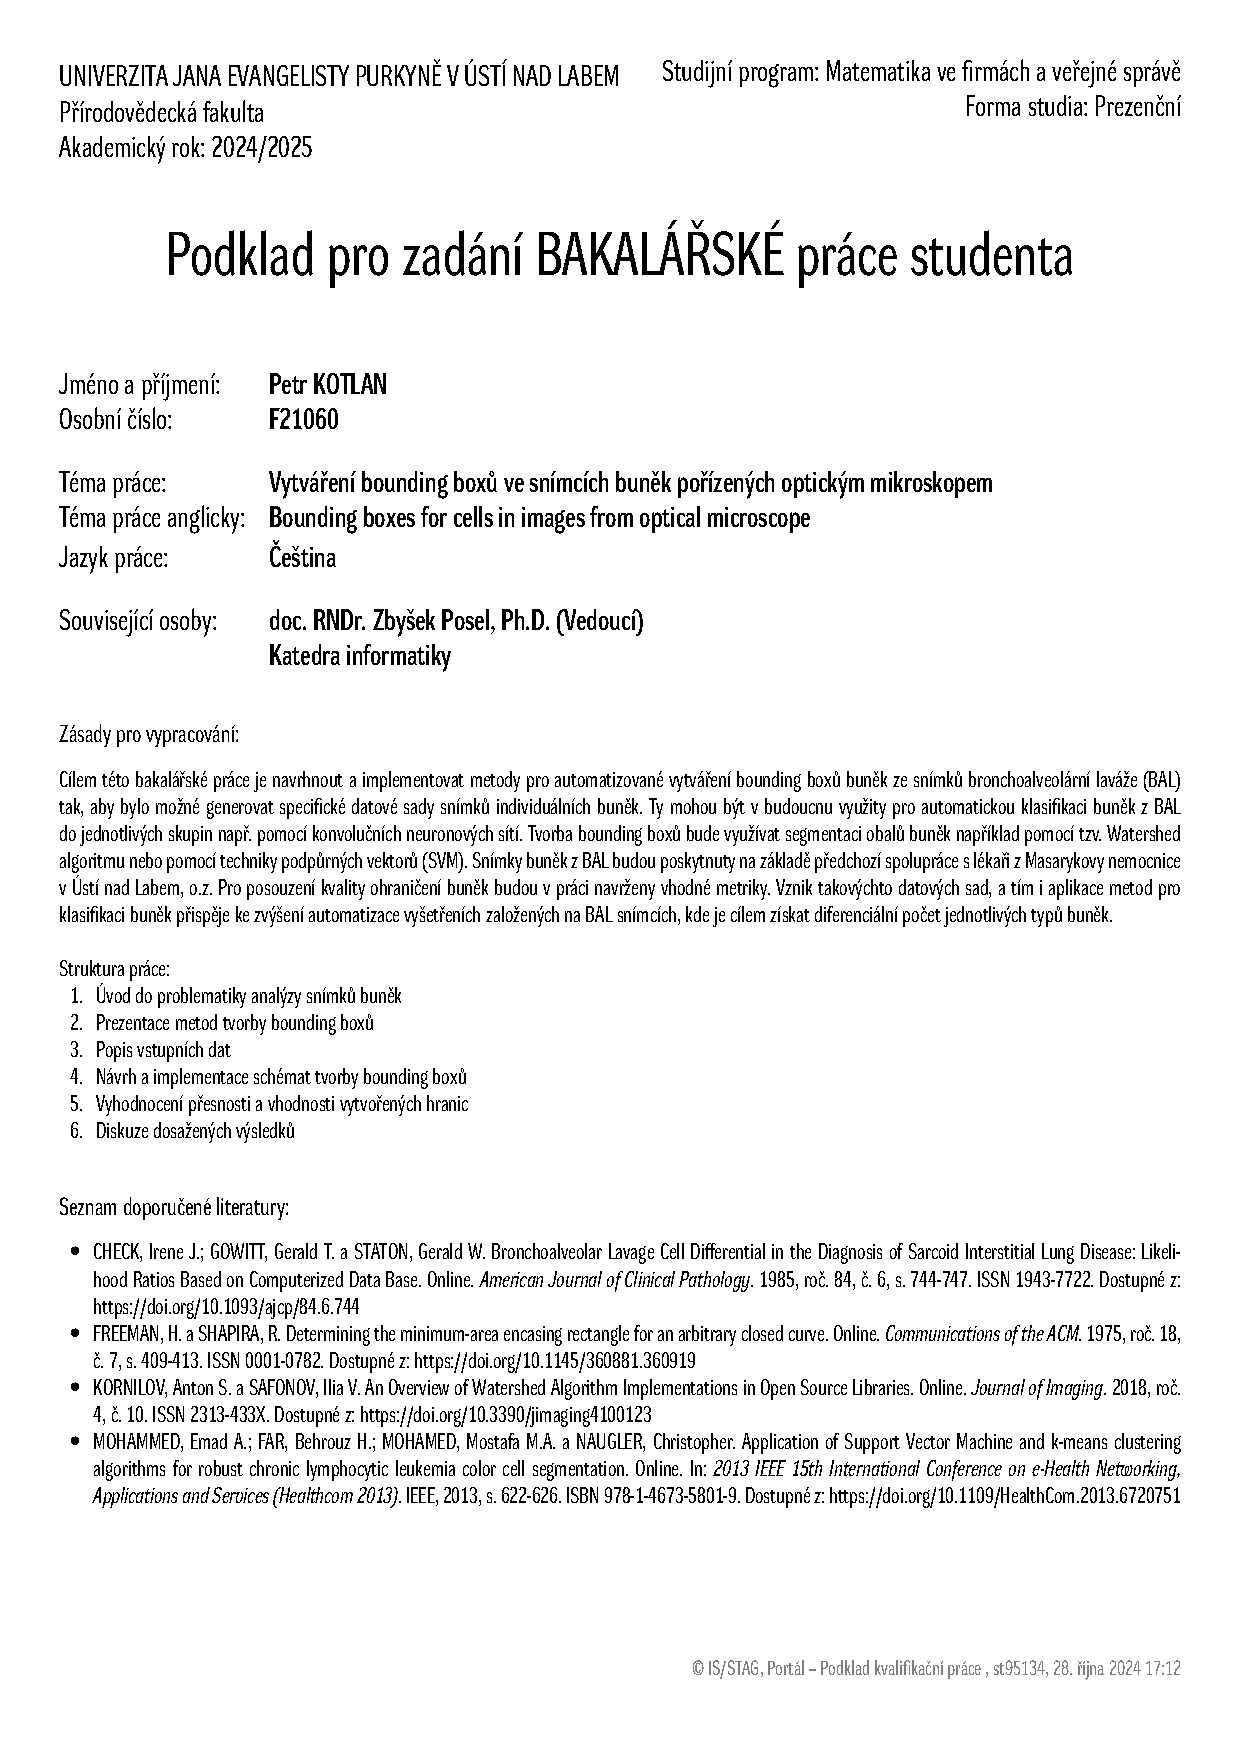
\includepdf[pages=-]{static/podklad_bp.pdf}
\thispagestyle{empty}
\addtocounter{page}{1} 

\textbf{Prohlášení}

\vspace{1cm}

Prohlašuji, že jsem tuto bakalářskou práci vypracoval samostatně a použil jen pramenů, které
cituji a uvádím v přiloženém seznamu literatury.

\vspace{0.5cm}

Byl jsem seznámen s tím, že se na moji práci vztahují práva a povinnosti vyplývající ze zákona
č. 121/2000 Sb., ve znění zákona č. 81/2005 Sb., autorský zákon, zejména se skutečností,
že Univerzita Jana Evangelisty Purkyně v Ústí nad Labem má právo na uzavření licenční
smlouvy o užití této práce jako školního díla podle § 60 odst. 1 autorského zákona, a s tím, že
pokud dojde k užití této práce mnou nebo bude poskytnuta licence o užití jinému subjektu,
je Univerzita Jana Evangelisty Purkyně v Ústí nad Labem oprávněna ode mne požadovat
přiměřený příspěvek na úhradu nákladů, které na vytvoření díla vynaložila, a to podle
okolností až do jejich skutečné výše.

\vspace{1cm}

\begin{multicols}{2}
    \begin{flushleft}
    V Ústí nad Labem dne ..............................
    \end{flushleft}

\newcolumn

\begin{flushright}
Podpis: ............................................
\end{flushright}


\end{multicols}

\newpage

\thispagestyle{empty}
\mbox{}
\newpage

\thispagestyle{empty}

% podekovani, vpravo dole
\null
\vfill

\begin{flushright}
    \textit{podekování}
\end{flushright}

\newpage

\thispagestyle{empty}
\mbox{}
\newpage

\thispagestyle{empty}

\textsc{Vytváření bounding boxů ve snímcích buněk pořízených optickým mikroskopem}

\vspace{0.5cm}

\textbf{Abstrakt}

\textbf{Klíčová slova}

\vspace{0.7cm}

\textsc{Bounding boxes for cells in images from optical microscope}

\textbf{Abstract}

\textbf{Keywords}

\newpage


\thispagestyle{empty}
\mbox{}
\newpage

\tableofcontents

\addcontentsline{toc}{chapter}{Úvod}

\newpage
\thispagestyle{empty}
\mbox{}
\newpage

\chapter*{Úvod}
\renewcommand{\chaptername}{Úvod}
uvod


\addcontentsline{toc}{chapter}{Seznam zdrojů}
\bibliographystyle{plain}
% \bibliography{bibliografie}
\begin{thebibliography}{4}

    \bibitem{Check19851201}
    CHECK, Irene J.; GOWITT, Gerald T. a STATON, Gerald W. Bronchoalveolar Lavage Cell Differential in the Diagnosis of Sarcoid Interstitial Lung Disease: Likelihood Ratios Based on Computerized Data Base. Online. \textit{American Journal of Clinical Pathology}. 1985, roč. 84, č. 6, s.~744-747. ISSN 1943-7722. Dostupné z: \url{https://doi.org/10.1093/ajcp/84.6.744}. [cit. 2024-09-20].
    \bibitem{Freeman1975}
    FREEMAN, H. a SHAPIRA, R. Determining the minimum-area encasing rectangle for an arbitrary closed curve. Online. \textit{Communications of the ACM}. 1975, roč. 18, č. 7, s.~409-413. ISSN 0001-0782. Dostupné z: \url{https://doi.org/10.1145/360881.360919}. [cit. 2024-09-20].
    \bibitem{Kornilov2018}
    KORNILOV, Anton S. a SAFONOV, Ilia V. An Overview of Watershed Algorithm Implementations in Open Source Libraries. Online. \textit{Journal of Imaging}. 2018, roč. 4, č. 10. ISSN 2313-433X. Dostupné z: \url{https://doi.org/10.3390/jimaging4100123}. [cit. 2024-09-20].
    \bibitem{Mohammed2013}
    MOHAMMED, Emad A.; FAR, Behrouz H.; MOHAMED, Mostafa M.A. a NAUGLER, Christopher. Application of Support Vector Machine and k-means clustering algorithms for robust chronic lymphocytic leukemia color cell segmentation. Online. In: \textit{2013 IEEE 15th International Conference on e-Health Networking, Applications and Services (Healthcom 2013)}. IEEE, 2013, s.~622-626. ISBN 978-1-4673-5801-9. Dostupné z: \url{https://doi.org/10.1109/HealthCom.2013.6720751}. [cit. 2024-09-20].
    
\end{thebibliography}
% \bibliography{bibliografie}

\end{document}